\documentclass[10pt]{beamer}

\newcommand{\mytitle}{Adding a third normal to CLUBB}
\newcommand{\myauthor}{Sven Bergmann}
\usepackage[utf8]{inputenc}
\usepackage{graphicx}
\usetheme{CambridgeUS}
\usecolortheme{dolphin}
\usepackage{bm}
\usepackage{tabularx}
\newcolumntype{Y}{>{\centering\arraybackslash}X}
\usepackage{diagbox}

\usepackage{appendixnumberbeamer}


% set colors
\definecolor{UWMyellow}{RGB}{255,189,0}
\setbeamercolor{block title}{bg=UWMyellow,fg=black}
\setbeamercolor{block body}{bg=UWMyellow!20,fg=black}
\setbeamercolor{block title alerted}{bg=black, fg=UWMyellow}
\setbeamercolor{block body alerted}{bg=black!20, fg=black}

\setbeamercolor*{block title example}{bg=UWMyellow, fg = black}
\setbeamercolor*{block body example}{bg=UWMyellow, fg = black}
\usebeamercolor[UWMyellow]{block title alerted}
\setbeamercolor*{palette primary}{bg=UWMyellow, fg = black}
\setbeamercolor*{palette secondary}{bg=UWMyellow, fg = black}
\setbeamercolor*{palette tertiary}{bg=UWMyellow, fg = black}
\setbeamercolor*{titlelike}{fg=black}
\setbeamercolor*{title}{bg=UWMyellow, fg=black}
\setbeamercolor*{item}{fg=UWMyellow}
\setbeamercolor*{caption name}{fg=black}
\usefonttheme{professionalfonts}

\hypersetup{
    pdftitle = {\mytitle},
    pdfauthor = {\myauthor}
}

\usepackage[style=alphabetic, backend=biber]{biblatex}
\addbibresource{include/bibliography.bib}

\usepackage[newfloat, outputdir=../auxil]{minted}
\usepackage{csquotes}
\newminted{python}{
    autogobble,
    frame=single,
    breaklines,
    fontsize=\footnotesize
}

\titlegraphic{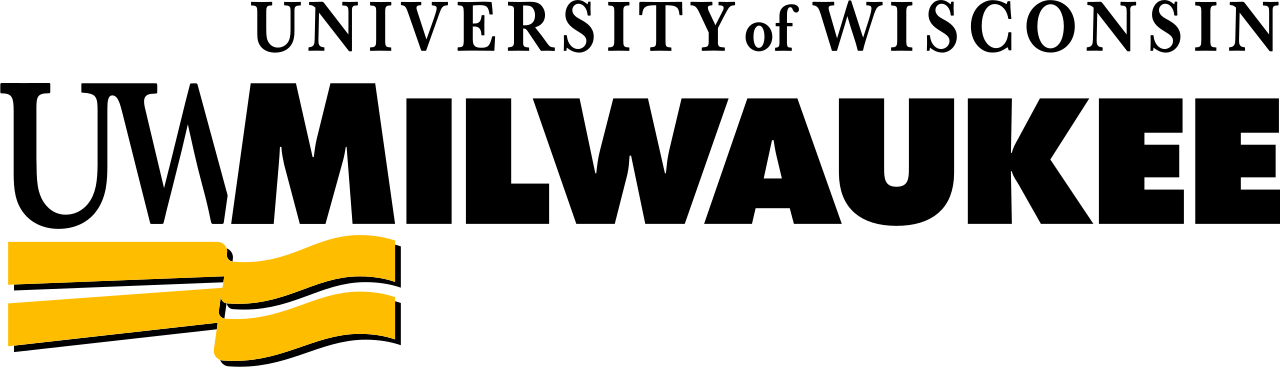
\includegraphics[height=1.5cm]{include/pictures/photo}}

\setbeamerfont{title}{size=\large}
\setbeamerfont{subtitle}{size=\small}
\setbeamerfont{author}{size=\small}
\setbeamerfont{date}{size=\small}
\setbeamerfont{institute}{size=\small}

\numberwithin{equation}{section}

\title{\mytitle}
\author[\myauthor]{\myauthor}
\institute[UWM]{University of Wisconsin Milwaukee}
\date[May 3, 2024]{May 3, 2024}

\AtBeginSection[]
{
    \begin{frame}{Contents}
        \tableofcontents[currentsection]
    \end{frame}
}

\newcommand{\wptwo}{ \overline{w'^2} }
\newcommand{\thlptwo}{ \overline{\theta_l'^2} }
\newcommand{\rtptwo}{ \overline{r_t'^2} }
\newcommand{\wpthlp}{ \overline{w' \theta_l'} }
\newcommand{\wprtp}{ \overline{w' r_t'} }
\newcommand{\rtpthlp}{ \overline{r_t' \theta_l'} }
\newcommand{\wptwothlp}{ \overline{w'^2 \theta_l'} }
\newcommand{\wptwortp}{ \overline{w'^2 r_t'} }
\newcommand{\wpthlptwo}{ \overline{w' \theta_l'^2} }
\newcommand{\wprtptwo}{ \overline{w' r_t'^2} }
\newcommand{\wprtpthlp}{ \overline{w' r_t' \theta_l'} }
\newcommand{\wpthree}{ \overline{w'^3} }
\newcommand{\thlpthree}{ \overline{\theta_l'^3} }
\newcommand{\rtpthree}{ \overline{r_t'^3} }
\newcommand{\wpfour}{ \overline{w'^4} }

\newcommand{\tsw}{{\tilde{\sigma}_w}}
\newcommand{\tswfact}{\left( 1 - \tilde{\sigma}_w^2 \right)}

\begin{document}

    \frame{\titlepage}

    \begin{frame}{Contents}
        \tableofcontents[hideallsubsections]
    \end{frame}


    \section{What is CLUBB?}\label{sec:what-is-clubb?}

    \begin{frame}{\textbf{C}loud \textbf{L}ayers \textbf{U}nified \textbf{B}y \textbf{B}inormals \ldots}
        \ldots is an atmospheric model that tries to predict the weather
        based on modeling a grid box with a sum of two normal distributions.
    \end{frame}


    \section{Introduction}\label{sec:introduction}

    \subsection{Motivation to add a third normal component}
    \label{subsec:motivation-to-add-a-third-normal-component}

    \begin{frame}
        \begin{large}
            Nature does not look like this, this is too binormal.
        \end{large}
        \begin{figure}[!htb]
            \centering
            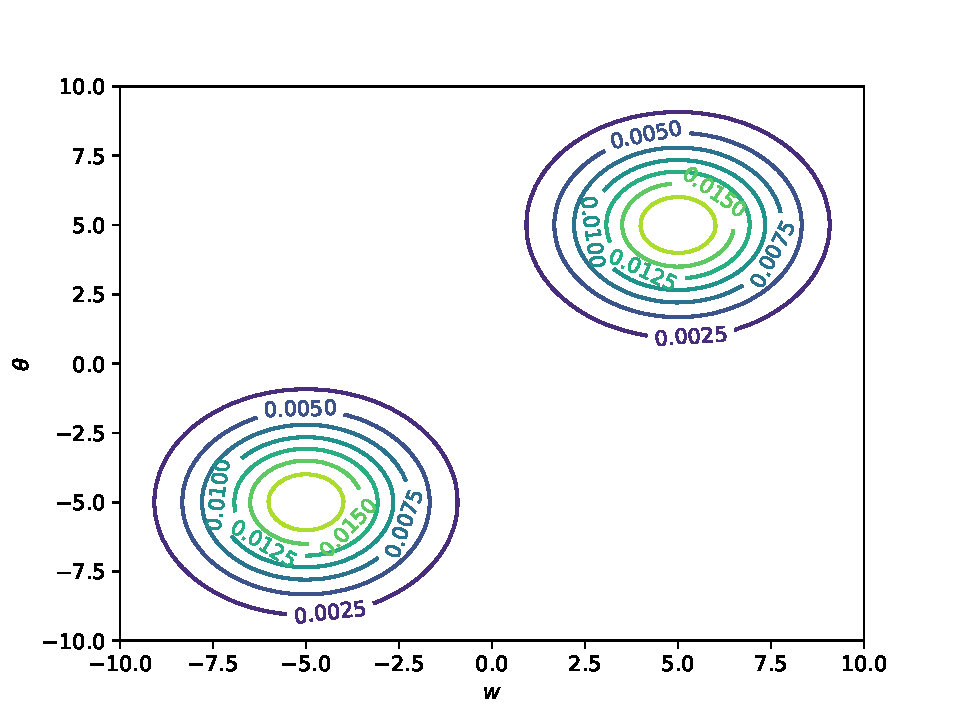
\includegraphics[width=.5\textwidth]{include/figures/plot1}
            \caption{Binormal plot for two strong up-/downdrafts}
            \label{fig:plot1}
            $w_1 = 5$, $w_2 = -5$, $\theta_{l1} = 5$, $\theta_{l2} = -5$,
            $\alpha = 0.5$, $\sigma_w = 2$, $\sigma_{\theta_{l1}} = 2$, $\sigma_{\theta_{l1}} = 2$.
        \end{figure}
    \end{frame}

    \begin{frame}
        \begin{large}
            To reduce the bimodality we can increase the widths.
        \end{large}
        \begin{figure}[!htb]
            \centering
            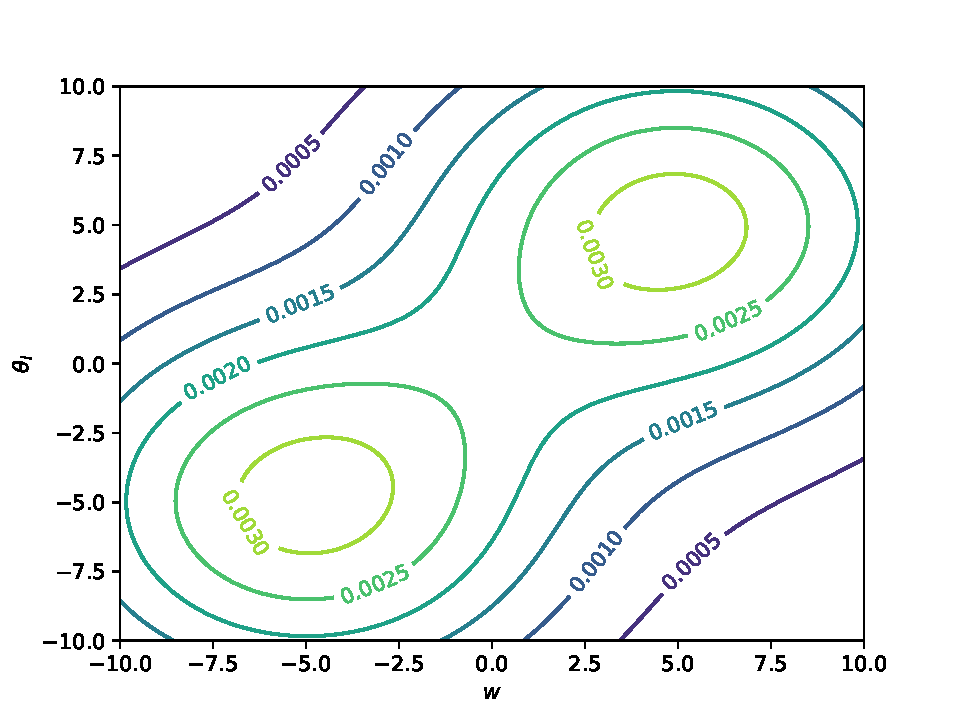
\includegraphics[width=.5\textwidth]{include/figures/plot2}
            \caption{Binormal plot for two strong up-/downdrafts with increased standard deviations}
            \label{fig:plot2}
            $w_1 = 5$, $w_2 = -5$, $\theta_{l1} = 5$, $\theta_{l2} = -5$,
            $\alpha = 0.5$, $\sigma_w = 5$, $\sigma_{\theta_{l1}} = 5$, $\sigma_{\theta_{l1}} = 5$.
        \end{figure}
    \end{frame}

    \begin{frame}
        \begin{large}
            Adding a third normal is more realistic.
        \end{large}
        \begin{figure}[!htb]
            \centering
            \begin{tabular}{cc}
                \multicolumn{1}{c}{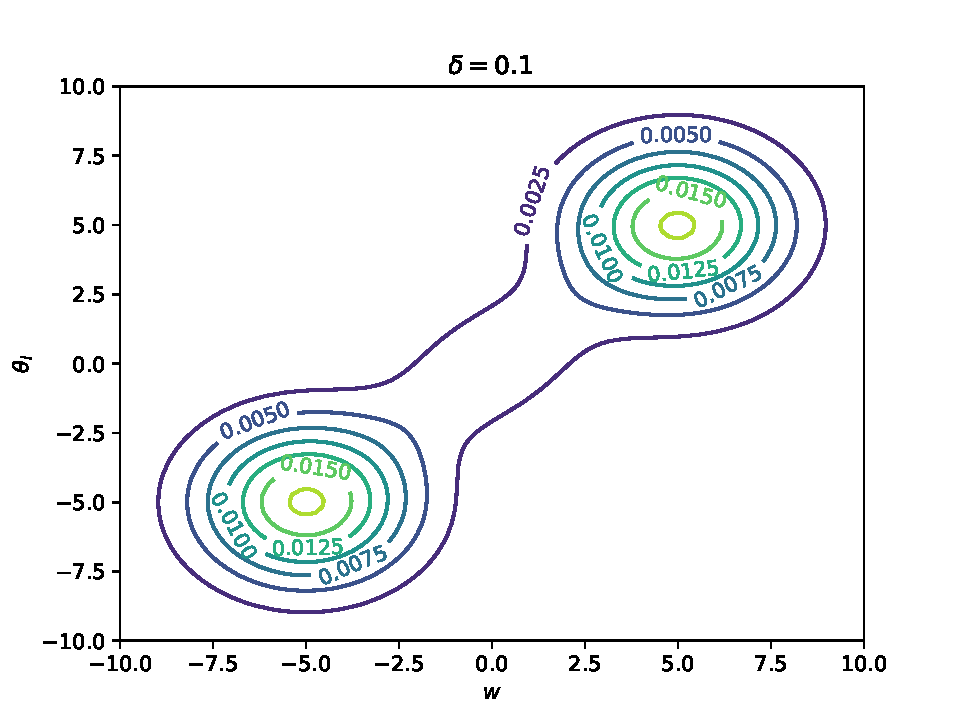
\includegraphics[width=0.3\textwidth]{include/figures/plot3_1}} &
                \multicolumn{1}{c}{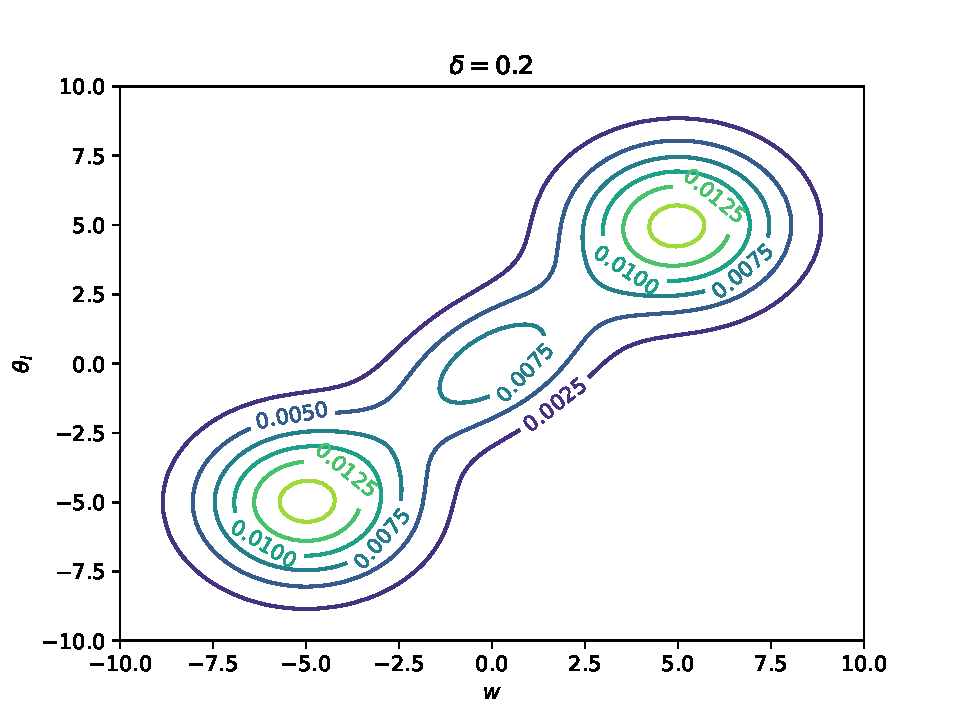
\includegraphics[width=0.3\textwidth]{include/figures/plot3_2}} \\
                \multicolumn{1}{c}{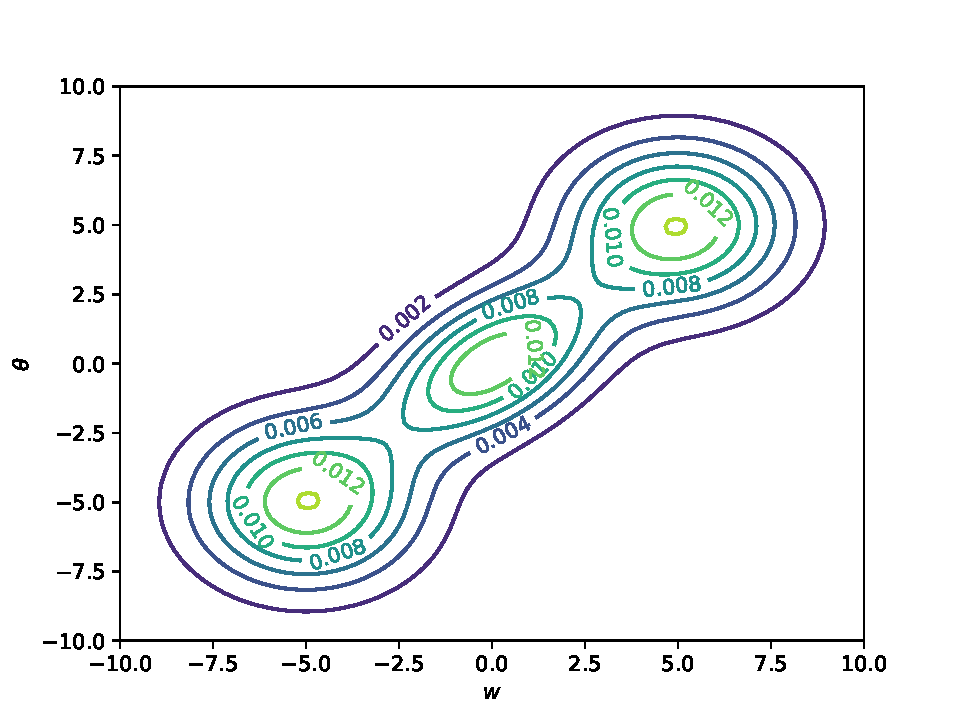
\includegraphics[width=0.3\textwidth]{include/figures/plot3_3}} &
                \multicolumn{1}{c}{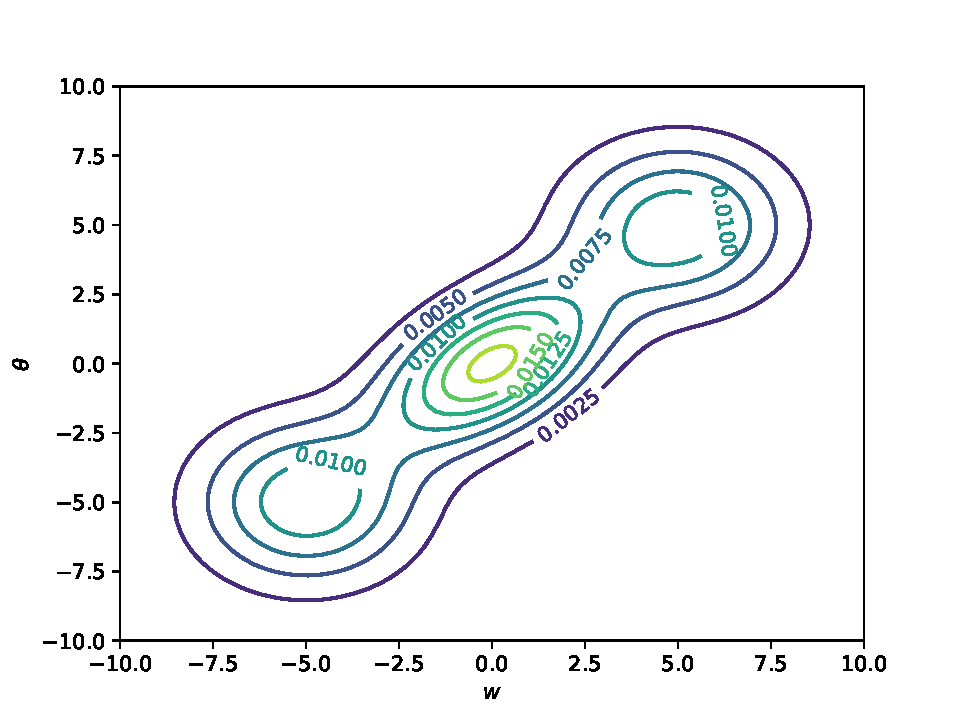
\includegraphics[width=0.3\textwidth]{include/figures/plot3_4}} \\
            \end{tabular}
            \caption{Trinormal plot for two strong up-/downdrafts with varying $\delta$}
            \label{fig:plot3}
            $w_1 = 5$, $w_2 = -5$, $\theta_{l1} = 5$, $\theta_{l2} = -5$,
            $\alpha = 0.5$, $\sigma_w = 2$, $\sigma_{\theta_{l1}} = 2$,  $\sigma_{\theta_{l2}} = 2$,
            $\sigma_{w3} = 2$, $\sigma_{3\theta_l} = 2$, $\rho_{w\theta_l} = 0.5$.
        \end{figure}
    \end{frame}

    \begin{frame}
        \begin{large}
            A third normal even allows \enquote{weird} shapes.
        \end{large}
        \begin{figure}[!htb]
            \centering
            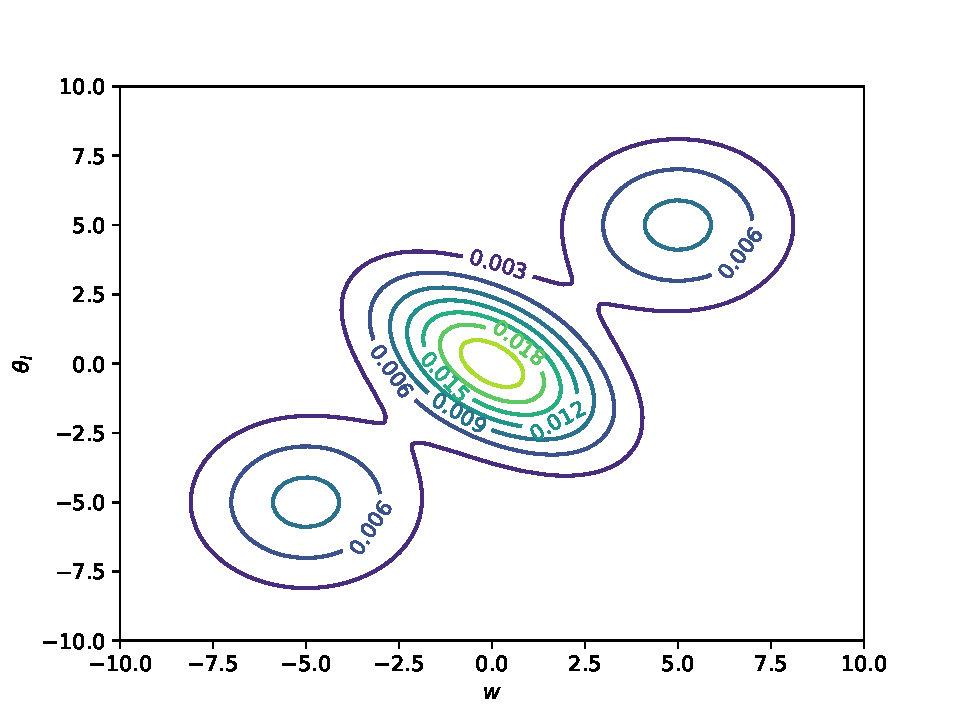
\includegraphics[width=.5\textwidth]{include/figures/plot4}
            \caption{Trinormal plot for two strong up-/downdrafts with a third peak in the middle}
            \label{fig:plot4}
            $w_1 = 5$, $w_2 = -5$, $\theta_{l1} = 5$, $\theta_{l2} = -5$,
            $\alpha = 0.5$, $\delta=0.5$, $\sigma_w = 2$, $\sigma_{\theta_{l1}} = 2$,
            $\sigma_{\theta_{l2}} = 2$, $\sigma_{w3} = 2$, $\sigma_{\theta_l 3} = 2$,
            $\rho_{w\theta_l} = 0.5$.
        \end{figure}
    \end{frame}

    \subsection{Closing turbulence pdes by integration over a pdf}
    \label{subsec:closing-turbulence-pdes-by-integration-over-a-pdf}

    \begin{frame}
        Consider the following prognostic pde~\autocite[p. 21]{larson2022clubbsilhs}:
        \begin{align*}
            \frac{\partial \wpthlp}{\partial t}
            &= -\overline{w}\frac{\partial \wpthlp}{\partial z}
            - \frac{1}{\rho_s} \frac{\partial \rho_s \wptwothlp}{\partial z}
            - \wptwo \frac{\partial \overline{\theta_l'}}{\partial z}
            - \wpthlp \frac{\partial \overline{w}}{\partial z}
            + \ldots
        \end{align*}
        We need to close the third order moment ($\wptwothlp$) by integration over the pdf.
    \end{frame}

    \subsection{Derivation of trinormal closures by transformation of binormal closures}
    \label{subsec:derivation-of-trinormal-closures-by-transformation-of-binormal-closures}

    \begin{frame}
        There already exist closures that assume a binormal pdf~\autocite{larson2005using}, e.g.
        \begin{align}
            \label{eq:wp2_bar_dGn}
            \wptwo
            &= \alpha [(w_1 - \overline{w})^2 + \sigma_w^2]
            + (1 - \alpha) [(w_2 - \overline{w})^2 + \sigma_w^2].
        \end{align}
    \end{frame}

    \begin{frame}
        We can transform to a trinormal pdf using the following formulas:
        \begin{align}
            \label{eq:w_prime_2_transform}
            \wptwo \frac{1 - \delta\lambda_w}{1 - \delta}
            &= \wptwo_{dGn}
        \end{align}
        \begin{align}
            \label{eq:w_prime_3_transform}
            \wpthree \frac{1}{1 - \delta}
            &= \wpthree_{dGn}
        \end{align}
        \begin{align}
            \label{eq:w_prime_3_div_w_prime_2_transform}
            \frac{\wpthree}{\wptwo^{3/2}} \frac{(1 - \delta)^{1/2}}{(1 - \lambda_w\delta)^{3/2}}
            &= \frac{\wpthree_{dGn}}{\wptwo_{dGn}^{3/2}}
        \end{align}
        \begin{align}
            \label{eq:theta_l_prime_transform}
            \thlptwo \frac{1 - \delta\lambda_\theta}{1 - \delta}
            &= \thlptwo_{dGn}
        \end{align}
        \begin{align}
            \label{eq:w_prime_theta_l_prime_transform}
            \wpthlp \frac{1 - \delta\lambda_{w\theta}}{1 - \delta}
            &= \wpthlp_{dGn}
        \end{align}
    \end{frame}

    \begin{frame}
        If we substitute in a formula for $\lambda_w$~\eqref{eq:lambda}, which will be explained later on, we get
        \begin{align}
            \wptwo \left(1 - \delta\frac{\sigma_{w 3}^2}{\wptwo}\right)
            &= (1 - \delta)\wptwo_{dGn} \\
            \iff \wptwo
            &= \wptwo_{dGn} - \delta\left(\wptwo_{dGn} - \sigma_{w 3}^2\right)
        \end{align}
    \end{frame}

    \begin{frame}
        \begin{table}[!htb]
            \centering
            \begin{tabularx}{\textwidth}{c|@{}Y@{}@{}Y@{}@{}Y@{}}
                \diagbox{$\sigma_{w 3}$}{$\delta$} & 0.1 & 0.5 & 0.9 \\
                \hline
                4
                & 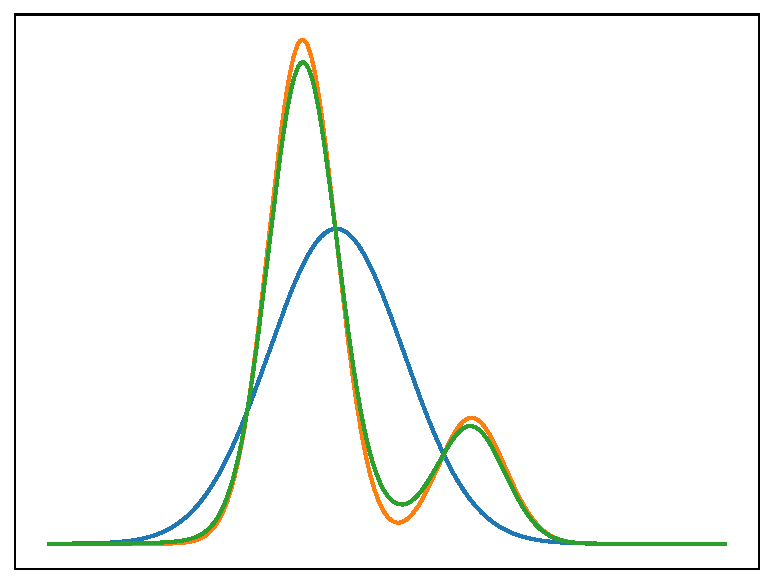
\includegraphics[width = .29\textwidth]{include/figures/1dplotslw40_delta1}
                & 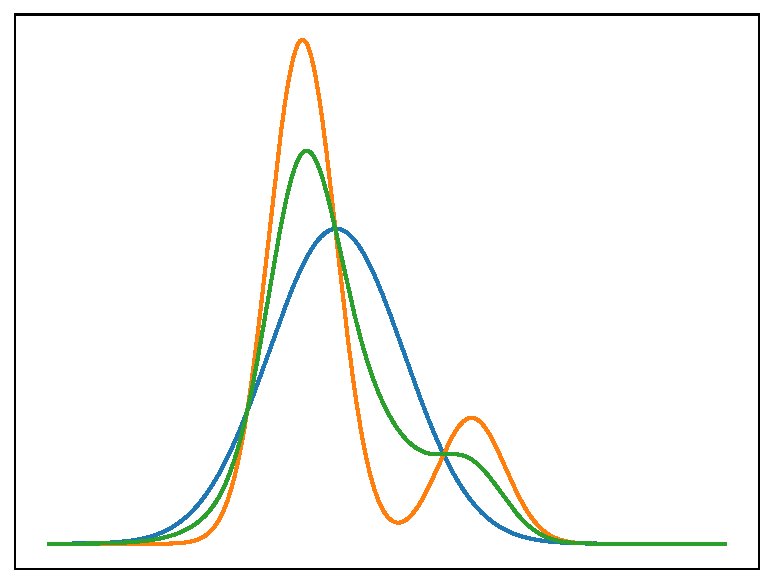
\includegraphics[width = .29\textwidth]{include/figures/1dplotslw40_delta5}
                & 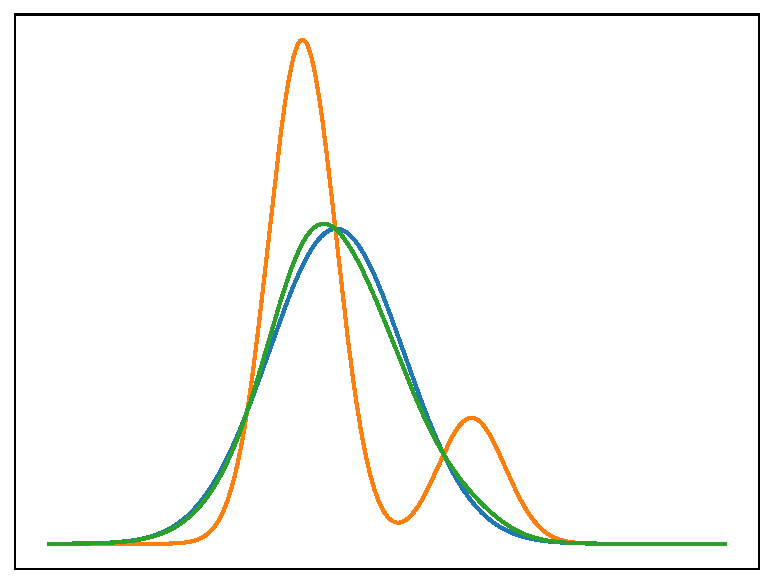
\includegraphics[width = .29\textwidth]{include/figures/1dplotslw40_delta9} \\
                \hline
                8
                & 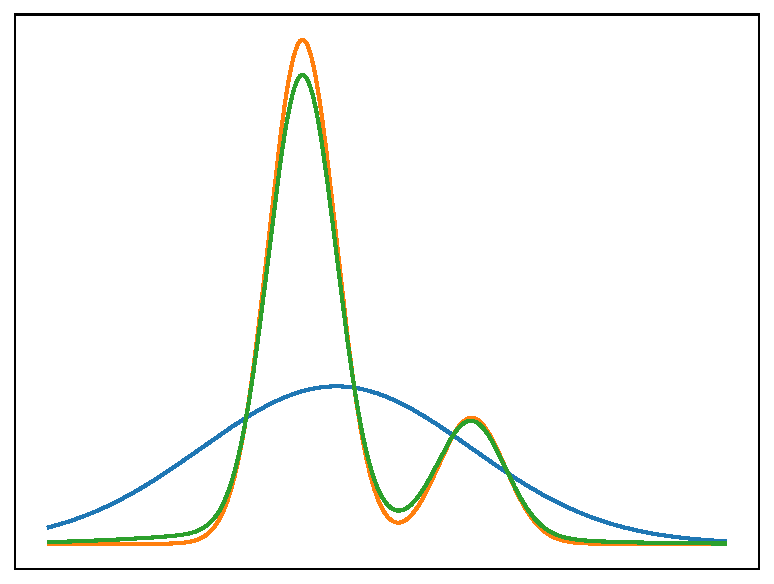
\includegraphics[width = .29\textwidth]{include/figures/1dplotslw80_delta1}
                & 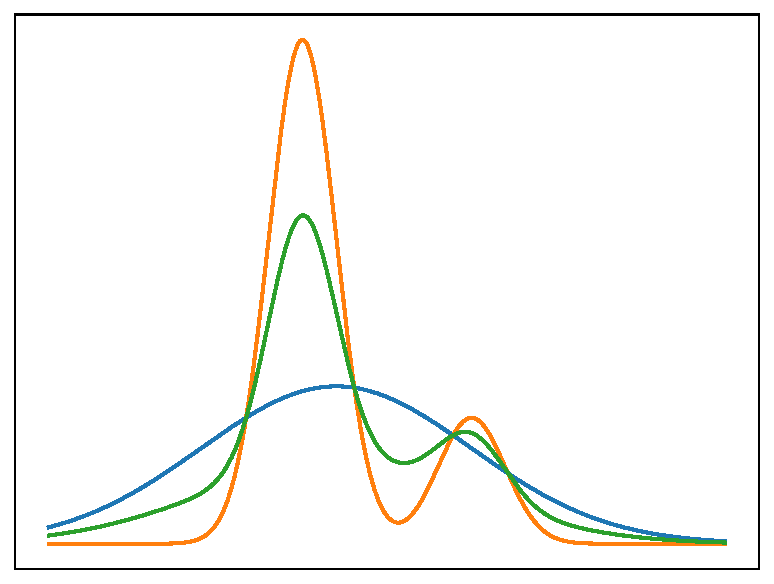
\includegraphics[width = .29\textwidth]{include/figures/1dplotslw80_delta5}
                & 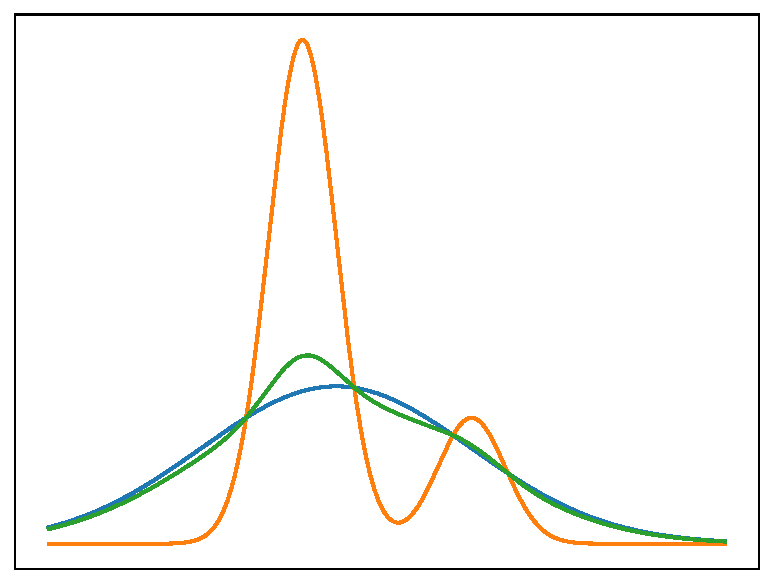
\includegraphics[width = .29\textwidth]{include/figures/1dplotslw80_delta9}
            \end{tabularx}
            \caption{1D Plots for different $\delta$ and $\sigma_{w3}$}
            $w_1 = 5$, $w_2 = -5$, $\alpha = 0.2$, $\sigma_w = 2$.
            The blue plot represents the third normal,
            the orange/red one represents the binormal,
            and the green one represents the mixture.
            The $x$ and $y$ labels and ticks are omitted for clarity.
            \label{tab:1dplotbitri}
        \end{table}
    \end{frame}

    \subsection{Goal}\label{subsec:goal}

    \begin{frame}
        The goal of this thesis is to verify that all the transformations work out well.
    \end{frame}

    \subsection{Inputs and Outputs}\label{subsec:inputs-and-outputs}

    \begin{frame}{Forward run (weather forecast)}
        \begin{itemize}
            [<+->]
            \item Given: $\overline{w}$, $\wptwo$, $\wpthree$, $\overline{\theta_l}$, $\wpthlp$,
            $\overline{r_t}$, $\wprtp$, $\thlptwo$, $\rtptwo$, $\rtpthlp$.
            \item Find: Parameters, which describe the shape of the underlying pdf,
            for ultimately describing higher-order moments,
            e.g. $\wptwothlp$ in terms of lower-order moments.
        \end{itemize}
    \end{frame}

    \begin{frame}{Backward run (verification direction)}
        \begin{itemize}
            [<+->]
            \item Given: pdf parameters, e.g.\ mean, standard deviation
            \item Find: lower- and higher-order moments
        \end{itemize}
    \end{frame}


    \section{Definitions}\label{sec:definitions}

    \subsection{Normal Distribution}\label{subsec:normal-distribution}



    \begin{frame}{Multivariate}
        We say that a random vector $\bm{X}$
        is distributed according to a multivariate normal distribution
        when it has the following joint density function~\autocite[p. 59]{izenman_modern_2008}:

        \begin{definition}[pdf of a multivariate normal distribution]
            \begin{align}
                f(\bm{x}| \bm{\mu}, \bm{\Sigma})
                = (2\pi)^{-\frac{r}{2}}
                \left|\bm{\Sigma}\right|^{-\frac{1}{2}}
                \exp\left(-\frac{1}{2}(\bm{x}-\bm{\mu})^\top \bm{\Sigma}^{-1} (\bm{x}-\bm{\mu})\right),
                \bm{x} \in \mathbb{R}^r,
            \end{align}
            where
            \begin{align}
                \bm{\mu} =
                \begin{pmatrix}
                    \mu_1  \\
                    \vdots \\
                    \mu_r
                \end{pmatrix}
                \in \mathbb{R}^r,
                \text{ and }
                \bm{\Sigma} =
                \begin{pmatrix}
                    \sigma_1^2                & \rho_{12}\sigma_1\sigma_2 & \ldots & \rho_{1r}\sigma_1\sigma_r \\
                    \rho_{12}\sigma_1\sigma_2 & \sigma_2^2                & \ldots & \vdots                    \\
                    \vdots                    & \ldots                    & \ddots & \vdots                    \\
                    \rho_{1r}\sigma_1\sigma_r & \ldots                    & \ldots & \sigma_r^2
                \end{pmatrix}
                \in \mathbb{R}^{r\times r}
            \end{align}
        \end{definition}
    \end{frame}

    \begin{frame}{Moments}
        We denote the skewness and kurtosis by the following:
        \begin{align}
            \mathbb{E}[X^3]
            &= \mathbb{E}\left[\left(\frac{X-\mu}{\sigma}\right)^3\right]
            = \frac{\mathbb{E}[(X-\mu)^3]}{(\mathbb{E}[(X-\mu)^2])^{3/2}}
            = \frac{\mu_3}{\sigma^3} \\
            \mathbb{E}[X^4]
            &= \mathbb{E}\left[\left(\frac{X-\mu}{\sigma}\right)^4\right]
            = \frac{\mathbb{E}[(X-\mu)^4]}{(\mathbb{E}[(X-\mu)^2])^2}
            = \frac{\mu_4}{\sigma^4}
        \end{align}
    \end{frame}

    \subsection{Variates of the pdf}\label{subsec:variates-of-the-pdf}

    \begin{frame}
        \begin{itemize}
            \item $w$ - upward wind (or up-/downdraft)
            \item $r_t$ - total water mixing ratio
            \item $\theta_l$ - liquid water potential temperature
        \end{itemize}
        \vspace{2cm}

        The variables mostly appear in centered form,
        e.g. $w' = w - \overline{w}$. \\
        For example $\wptwo$ is the centered variance.
    \end{frame}


    \section{Definition of the trinormal distribution, \texorpdfstring{$P_{tmg}$}{P tmg}}
    \label{sec:definition-of-the-trinormal-distribution-p_tmg}

    \begin{frame}{Normal Mixture}
        \begin{align}
            \label{eq:normal_mix_pdf}
            P_{tmg}(w, \theta_l, r_t)
            &= \alpha (1-\delta) \mathcal{N}(\mu_1, \Sigma_1) \nonumber\\
            &\quad+ (1-\alpha) (1-\delta) \mathcal{N}(\mu_2, \Sigma_2) \nonumber\\
            &\quad+ \delta \mathcal{N}(\mu_3, \Sigma_3),
        \end{align}
        where $\mathcal{N}$ denotes the multivariate normal distribution,
        $\alpha \in (0,1)$ is the mixture fraction of the binormal,
        and $\delta \in [0,1)$ is the weight of the third normal.
    \end{frame}

    \begin{frame}{Mean of first and second component}
        \begin{align}
            \mu_1 =
            \begin{pmatrix}
                w_1         \\
                \theta_{l1} \\
                r_{t1}
            \end{pmatrix},
            \mu_2 =
            \begin{pmatrix}
                w_2         \\
                \theta_{l2} \\
                r_{t2}
            \end{pmatrix}
        \end{align}
    \end{frame}

    \begin{frame}{Covariance matrices of first and second component}
        \begin{align}
            \Sigma_1 =
            \begin{pmatrix}
                \sigma_w^2 & 0                                                      & 0                                                      \\
                0          & \sigma_{\theta_{l1}}^2                                 & \rho_{\theta_l r_t} \sigma_{\theta_l 3} \sigma_{r_t 3} \\
                0          & \rho_{\theta_l r_t} \sigma_{\theta_l 3} \sigma_{r_t 3} & \sigma_{r_{t1}}^2
            \end{pmatrix}
        \end{align}
        \begin{align}
            \Sigma_2 =
            \begin{pmatrix}
                \sigma_w^2 & 0                                                      & 0                                                      \\
                0          & \sigma_{\theta_{l2}}^2                                 & \rho_{\theta_l r_t} \sigma_{\theta_l 3} \sigma_{r_t 3} \\
                0          & \rho_{\theta_l r_t} \sigma_{\theta_l 3} \sigma_{r_t 3} & \sigma_{r_{t2}}^2
            \end{pmatrix}
        \end{align}
    \end{frame}

    \begin{frame}{Placing of the third component}
        We place the third normal component at the mean in order to simplify the math.
        \begin{align}
            \mu_3 =
            \begin{pmatrix}
                \overline{w}        \\
                \overline{\theta_l} \\
                \overline{r_t}
            \end{pmatrix},
            \text{ and }
            \Sigma_3 =
            \begin{pmatrix}
                \sigma_{w 3}^2 &
                \rho_{w \theta_l 3} \sigma_{w 3} \sigma_{\theta_l 3} &
                \rho_{w r_t 3} \sigma_{w 3} \sigma_{r_t 3} \\
                \rho_{w \theta_l 3} \sigma_{w 3} \sigma_{\theta_l 3} &
                \sigma_{\theta_l 3}^2 &
                \rho_{\theta_l r_t 3} \sigma_{\theta_l 3} \sigma_{r_t 3} \\
                \rho_{w r_t 3} \sigma_{w 3} \sigma_{r_t 3} &
                \rho_{\theta_l r_t 3} \sigma_{\theta_l 3} \sigma_{r_t 3} &
                \sigma_{r_t 3}^2
            \end{pmatrix}
        \end{align}
    \end{frame}

    \begin{frame}{Additional definitions}
        \begin{align}
            \label{eq:lambda}
            \lambda_w \equiv \frac{\sigma_{w 3}^2}{\wptwo}, \quad
            \lambda_\theta \equiv \frac{\sigma_{\theta_l 3}^2}{\thlptwo}, \quad
            \lambda_r \equiv \frac{\sigma_{r_t 3}^2}{\rtptwo},
        \end{align}
        \begin{align}
            \label{eq:lambda_two}
            \lambda_{\theta r} \equiv
            \frac{\rho_{\theta_l r_t} \sigma_{\theta_l 3} \sigma_{r_t 3}}{\rtpthlp}, \quad
            \lambda_{w \theta} \equiv
            \frac{\rho_{w \theta_l} \sigma_{w 3} \sigma_{\theta_l 3}}{\wpthlp}, \quad
            \lambda_{w r} \equiv
            \frac{\rho_{w r_t} \sigma_{w 3} \sigma_{r_t 3}}{\wprtp}
        \end{align}
    \end{frame}


    \section{Formulas for higher-order moments}\label{sec:formulas-for-higher-order-moments}

    \begin{frame}
        \begin{align}
            \label{eq:wp4}
            \wpfour
            &= \left(\wptwo\right)^2
            \frac{(1-\delta \lambda_w)^2}{(1-\delta)}
            \left(3 \tsw^4 + 6 \tswfact \tsw^2 + \tswfact^2\right) \nonumber\\
            &+ \frac{1}{\tswfact} \frac{1}{(1-\delta \lambda_w)}
            \frac{\left(\wpthree\right)^2}{\wptwo} \nonumber\\
            &+ \delta 3 \lambda_w^2 \left(\wptwo\right)^2
        \end{align}
    \end{frame}

    \begin{frame}
        \begin{align}
            \label{eq:wp2thlp_solved}
            \wptwothlp
            &= \frac{1}{\tswfact} \frac{1 - \delta \lambda_{w\theta}}{1-\delta \lambda_w} \frac{\wpthree}{\wptwo} \wpthlp
        \end{align}
    \end{frame}

    \begin{frame}
        \begin{align}
            \label{eq:wpthlp2_solved}
            \wpthlptwo
            &= \frac{2}{3} \frac{(1-\delta \lambda_{w \theta})^2}{(1-\delta \lambda_w)^2} \frac{1}{\tswfact^2} \frac{\wpthree}{\left(\wptwo \right)^2} \left(\wpthlp \right)^2 \nonumber\\
            &+ \frac{1}{3} \frac{(1-\delta \lambda_w)}{(1-\delta \lambda_{w \theta})} \tswfact \frac{\wptwo \; \thlpthree}{\wpthlp}
        \end{align}
    \end{frame}


    \section{Asymptotics}\label{sec:asymptotics}

    \begin{frame}{Limit for \texorpdfstring{$\wpfour$}{wprime4bar} as \texorpdfstring{$\delta$}{delta} goes to 1}
        As skewness goes to zero we want the pdf to revert to a single normal ($\delta \to 1$).
        \begin{align}
            \label{eq:limit_wprime4_delta_to_1}
            \lim_{\substack{\delta \to 1, \\ \wpthree \to 0}}
            \left(\wpfour\right)
            = 3 \left(\wptwo\right)^2
        \end{align}
    \end{frame}

    \begin{frame}{Limit for \texorpdfstring{$\wptwothlp$}{wprime2thetalbar} as \texorpdfstring{$\delta$}{delta} goes to 1}
        As skewness goes to zero we want the pdf to revert to a single normal ($\delta \to 1$).
        \begin{align}
            \label{eq:limit_wprime2thetalbar_delta_to_1}
            \lim_{\delta \to 1}\left(\wptwothlp\right)
            = \frac{(c_1 - 2)^2 \wpthlp \cdot \wpthree}{(c_2 - 2)\left((c_1 - 2)\wptwo + \sigma_w^2\right)}
        \end{align}
    \end{frame}

    \begin{frame}{Limit for \texorpdfstring{$\wptwothlp$}{wprimethetaltwobar} as \texorpdfstring{$\delta$}{delta} goes to 1}
        As skewness goes to zero we want the pdf to revert to a single normal ($\delta \to 1$).
        \begin{align}
            \label{eq:limit_wprimethetalprime2bar_delta_to_1}
            \lim_{\delta \to 1}\left(\wptwothlp\right)
            =
            \frac{1}{3}
            \left(
            \frac{
                2 \wpthree \left(\wpthlp \right)^2
            }
            {
                \left(\wptwo^2 - 2 \wptwo \frac{\sigma_w^2}{2 - c_1} + \left(\frac{\sigma_w^2}{2 - c_1}\right)^2 \right)
            }
            \right.
            \nonumber\\
            +
            \left.
            \frac{\thlpthree \; \wptwo(2 - c_2)}{\wpthlp(2 - c_1)}
            -
            \frac{\sigma_w^2 \thlpthree}{\wpthlp (2 - c_2)}
            \right)
        \end{align}
    \end{frame}


    \section{Integration using SymPy}\label{sec:integration-using-sympy}

    \begin{frame}
        \begin{center}
            We have checked the higher-order moment formulas using SymPy.\\
            \vspace{3cm}
            \textbf{DEMONSTRATION} \\
            (Analytic integration using SymPy~\autocite{10.7717/peerj-cs.103})
        \end{center}
    \end{frame}

    \begin{frame}[allowframebreaks, fragile]{Code to follow along the demonstration}
        \begin{listing}[!ht]
            \caption{Import statements}
            \label{lst:import}
            \begin{pythoncode}
                import sympy as sp
                from IPython.display import display
                from sympy import abc, oo, Symbol, Integral
                from sympy.stats import Normal, density
            \end{pythoncode}
        \end{listing}

        \begin{listing}[!ht]
            \caption{Defining symbols}
            \label{lst:defsymb}
            \begin{pythoncode}
                sigma_w = Symbol('\\sigma_w')
                w_1 = Symbol('w_1')
                w_2 = Symbol('w_2')
                w_bar = Symbol('\\overline{w}')
                sigma_w_3 = Symbol('\\sigma_{w3}')
                w_prime_2_bar = Symbol('\\overline{w\'^2}')
            \end{pythoncode}
        \end{listing}

        \begin{listing}[!ht]
            \caption{Defining the marginals}
            \label{lst:defmarginals}
            \begin{pythoncode}
                G_1_w = Normal(name='G_1_w', mean=w_1, std=sigma_w)
                G_1_w_density = density(G_1_w)(sp.abc.w)
                G_2_w = Normal(name='G_2_w', mean=w_2, std=sigma_w)
                G_2_w_density = density(G_2_w)(sp.abc.w)
                G_3_w = Normal(name='G_3_w', mean=w_bar, std=sigma_w_3)
                G_3_w_density = density(G_3_w)(sp.abc.w)
                G_w = ((1 - sp.abc.delta) * sp.abc.alpha * G_1_w_density +
                    (1 - sp.abc.delta) * (1 - sp.abc.alpha) * G_2_w_density +
                    sp.abc.delta * G_3_w_density)
            \end{pythoncode}
        \end{listing}

        \begin{listing}[!ht]
            \caption{Defining and displaying the needed integral}
            \label{lst:intwp2bar}
            \begin{pythoncode}
                w_prime_2_bar_int = sp.Integral((sp.abc.w - w_bar) ** 2 * G_w, [sp.abc.w, -oo, oo])
                display(sp.Eq(w_prime_2_bar, w_prime_2_bar_int))
            \end{pythoncode}
        \end{listing}

        \begin{listing}[!ht]
            \caption{Calculating and printing the integral}
            \label{lst:intwp2barcalc}
            \begin{pythoncode}
                w_prime_2_bar_int_val = w_prime_2_bar_int.doit(conds='none').simplify()
                display(sp.Eq(w_prime_2_bar, w_prime_2_bar_int_val))
            \end{pythoncode}
        \end{listing}

        \begin{listing}[!ht]
            \caption{Python function for the second order moment}
            \label{lst:intwp2barsym}
            \begin{pythoncode}
                def w_prime_2_bar_check(delta=sp.abc.delta, alpha=sp.abc.alpha, w_1=w_1, w_2=w_2, w_bar=w_bar, sigma_w=sigma_w, sigma_w_3=sigma_w_3):
                return (((1 - delta) * alpha * ((w_1 - w_bar) ** 2 + sigma_w ** 2))
                    + ((1 - delta) * (1 - alpha) * ((w_2 - w_bar) ** 2 + sigma_w ** 2))
                    + (delta * sigma_w_3 ** 2))
            \end{pythoncode}
        \end{listing}

        \begin{listing}[!ht]
            \caption{Printing the symbolic equation}
            \label{lst:intwp2barsymprint}
            \begin{pythoncode}
                display(sp.Eq(w_prime_2_bar, w_prime_2_bar_check()))
            \end{pythoncode}
        \end{listing}

        \begin{listing}[!ht]
            \caption{Check if the integral and the given formula are the same}
            \label{lst:intwp2barfinalcheck}
            \begin{pythoncode}
                display(sp.factor(sp.Eq(w_prime_2_bar_int_val, w_prime_2_bar_check()), sp.abc.alpha, sp.abc.delta))
            \end{pythoncode}
        \end{listing}
    \end{frame}

    \begin{frame}{References}
        \printbibliography
    \end{frame}

    \appendix

    \begin{frame}
        We say that a random variable $X$ is distributed
        according to a normal distribution ($X \sim \mathcal{N}(\mu, \sigma^2)$) when it has the following pdf:

        \begin{definition}[pdf of a normal distribution]
            \begin{align}
                \label{eq:pdf_normal_dist}
                f(x|\mu, \sigma^2) = \frac{1}{\sqrt{2\pi\sigma^2}}
                \exp{\left(-\frac{1}{2}\left(\frac{x-\mu}{\sigma}\right)^2\right)}
            \end{align}
        \end{definition}
    \end{frame}

    \begin{frame}[allowframebreaks]

        Considering that the skewness goes to zero ($Sk_w \to 0$),
        we want the pdf to revert to a single normal distribution.
        Therefore, we need
        \begin{align}
            \delta, \lambda_w, \lambda_r, \lambda_\theta,
            \lambda_{w r}, \lambda_{w \theta}, \lambda_{\theta r}
            \to 1.
        \end{align}
        In this limit, there are no third-order moments anymore, so they have to go to 0 as well.
        Also, we want to have that the kurtosis is approaching 3 (value of the kurtosis of a standard normal distribution).
        To ensure those points, as well as no division by zero in the code, we can define the following properties:
        \begin{align}
            \label{eq:delta_propto}
            \lim_{\delta \to 1} (1-\delta) \propto |Sk_w|,
        \end{align}
        which means that in the limit as $\delta \to 1$,
        $(1-\delta)$ should \enquote{behave as} the absolute value of the skewness of $w$,
        \begin{align}
            0 < \lim_{\delta\to 1} \left(\frac{1-\delta\lambda_x}{1-\delta}\right) < \infty,
        \end{align}
        where $x$ means any of $w$, $r_t$, or $\theta_l$,
        \begin{align}
            0 < \lim_{\delta\to 1} \left(\frac{1-\delta\lambda_x}{1-\delta\lambda_y}\right) < \infty
        \end{align}
        where $x$ is the same as above and $y$ means any of $w$, $r_t$, or $\theta_l$, $x \neq y$,
        \begin{align}
            0 < \lim_{\delta \to 1} \left(\tsw\right)^2
            = \lim_{\delta \to 1} \left(\frac{\sigma_w^2}{\wptwo} \frac{1-\delta}{1-\delta \lambda_w}\right) < 1.
        \end{align}
        To ensure~\eqref{eq:delta_propto}, we can use a linear \enquote{fit}, which looks like
        \begin{align}
            \label{eq:lambda_fit}
            \lambda_w = \lambda_\theta = \lambda_q
            = (1 - c_1) \delta + c_1,
        \end{align}
        where $c_1$ is some constant.
        The fit for the other $\lambda$'s is
        \begin{align}
            \label{eq:lambda_xy_fit}
            \lambda_{w\theta} = \lambda_{q\theta} = \lambda_{wq}
            = (1 - c_2) \delta + c_2,
        \end{align}
        where again $c_2$ is some constant.
        Note, that we already have a definition for the $\lambda$'s (\eqref{eq:lambda}).
        This definition is just for the backward run though,
        because we actually have to choose $\lambda$ in the forward direction.

        If we now look at the limit with the proposed fit (\eqref{eq:lambda_fit}),
        where $x$ is one of the three variates, we get:
        \begin{align}
            \lim_{\delta \to 1} \left(\frac{1 - \delta\lambda_x}{1 - \delta}\right)
            &= \lim_{\delta \to 1} \left(\frac{1 - \delta((1 - c_1) \delta + c_1)}{1 - \delta}\right)
            = \lim_{\delta \to 1} \left(\frac{1 - ((1 - c_1) \delta^2 + c_1\delta)}{1 - \delta}\right) \\
            &= \lim_{\delta \to 1} \left(\frac{1 - \delta^2 + c_1\delta^2 - c_1\delta}{1 - \delta}\right)
            = \lim_{\delta \to 1} \left(\frac{1 - \delta^2 + c_1\delta(\delta - 1)}{1 - \delta}\right) \\
            &= \lim_{\delta \to 1} \left(\frac{1 - \delta^2}{1 - \delta}\right)
            - \lim_{\delta \to 1} \left(\frac{c_1\delta(1 - \delta)}{1 - \delta}\right) \\
            \text{(L'Hôpital)}
            &\overset{\left[\frac{0}{0}\right]}{=} \lim_{\delta \to 1} \left(\frac{-2\delta}{-1}\right)
            - \lim_{\delta \to 1} \left(c_1\delta\right) \\
            &= 2 - c_1.
        \end{align}
        Then, we can also define the range of $c_1$,
        which should be $(0, 2)$ because we want to have $0 < \delta\lambda_w < 1$.
        For the reciprocal, we then have
        \begin{align}
            \lim_{\delta \to 1} \left(\frac{1 - \delta}{1 - \delta\lambda_x}\right)
            &= \lim_{\delta \to 1} \left(\frac{1 - \delta}{1 - \delta^2 + c_1\delta^2 - c_1\delta}\right)
            \overset{\left[\frac{0}{0}\right]}{=} \lim_{\delta \to 1} \left(\frac{-1}{- 2\delta + 2c_1\delta - c_1}\right) \\
            &= \frac{-1}{-2 + c_1} = \frac{1}{2 - c_1}.
        \end{align}
    \end{frame}

\end{document}